% !TeX document-id = {c68f4be8-c497-43e0-82df-e9ebfbea9577}
% !TeX TXS-program:pdflatex = pdflatex -synctex=1 -interaction=nonstopmode --shell-escape %.tex
% новая команда \RNumb для вывода римских цифр
\documentclass[a4paper,14pt]{extarticle}
\usepackage{amssymb}
\usepackage{amsmath}
\usepackage{amsthm}
\usepackage{caption}
\usepackage{misccorr}
\usepackage[noadjust]{cite}
\usepackage{cmap}
\usepackage[utf8x]{inputenc}
\usepackage[T2A]{fontenc}
\usepackage[english, russian]{babel}
\usepackage{graphics}
\usepackage{graphicx}
\usepackage{textcomp}
\usepackage{verbatim}
\usepackage{makeidx}
\usepackage{geometry}
\usepackage{float}
\usepackage{bm}
\usepackage{esint}
\usepackage{mathtools}
\usepackage{graphicx}
\usepackage{listings}
\usepackage{courier}
\usepackage{multirow}
\usepackage{graphicx}
\usepackage{xcolor}
\usepackage{ucs}

\usepackage{threeparttable}
\usepackage{csvsimple}
\usepackage{longtable,ltcaption,booktabs}
\usepackage{tabularx}


\lstdefinestyle{asm}{
	language={[x86masm]Assembler},
	backgroundcolor=\color{white},
	basicstyle=\footnotesize\ttfamily,
	keywordstyle=\color{blue},
	stringstyle=\color{red},
	commentstyle=\color{gray},
	numbers=left,
	numberstyle=\tiny,
	stepnumber=1,
	numbersep=5pt,
	frame=single,
	tabsize=4,
	captionpos=b,
	breaklines=true
}

\lstset{basicstyle=\fontsize{10}{10}\selectfont,breaklines=true,inputencoding=utf8x,extendedchars=\true}

\lstset{
	literate=
	{а}{{\selectfont\char224}}1
	{б}{{\selectfont\char225}}1
	{в}{{\selectfont\char226}}1
	{г}{{\selectfont\char227}}1
	{д}{{\selectfont\char228}}1
	{е}{{\selectfont\char229}}1
	{ё}{{\"e}}1
	{ж}{{\selectfont\char230}}1
	{з}{{\selectfont\char231}}1
	{и}{{\selectfont\char232}}1
	{й}{{\selectfont\char233}}1
	{к}{{\selectfont\char234}}1
	{л}{{\selectfont\char235}}1
	{м}{{\selectfont\char236}}1
	{н}{{\selectfont\char237}}1
	{о}{{\selectfont\char238}}1
	{п}{{\selectfont\char239}}1
	{р}{{\selectfont\char240}}1
	{с}{{\selectfont\char241}}1
	{т}{{\selectfont\char242}}1
	{у}{{\selectfont\char243}}1
	{ф}{{\selectfont\char244}}1
	{х}{{\selectfont\char245}}1
	{ц}{{\selectfont\char246}}1
	{ч}{{\selectfont\char247}}1
	{ш}{{\selectfont\char248}}1
	{щ}{{\selectfont\char249}}1
	{ъ}{{\selectfont\char250}}1
	{ы}{{\selectfont\char251}}1
	{ь}{{\selectfont\char252}}1
	{э}{{\selectfont\char253}}1
	{ю}{{\selectfont\char254}}1
	{я}{{\selectfont\char255}}1
	{А}{{\selectfont\char192}}1
	{Б}{{\selectfont\char193}}1
	{В}{{\selectfont\char194}}1
	{Г}{{\selectfont\char195}}1
	{Д}{{\selectfont\char196}}1
	{Е}{{\selectfont\char197}}1
	{Ё}{{\"E}}1
	{Ж}{{\selectfont\char198}}1
	{З}{{\selectfont\char199}}1
	{И}{{\selectfont\char200}}1
	{Й}{{\selectfont\char201}}1
	{К}{{\selectfont\char202}}1
	{Л}{{\selectfont\char203}}1
	{М}{{\selectfont\char204}}1
	{Н}{{\selectfont\char205}}1
	{О}{{\selectfont\char206}}1
	{П}{{\selectfont\char207}}1
	{Р}{{\selectfont\char208}}1
	{С}{{\selectfont\char209}}1
	{Т}{{\selectfont\char210}}1
	{У}{{\selectfont\char211}}1
	{Ф}{{\selectfont\char212}}1
	{Х}{{\selectfont\char213}}1
	{Ц}{{\selectfont\char214}}1
	{Ч}{{\selectfont\char215}}1
	{Ш}{{\selectfont\char216}}1
	{Щ}{{\selectfont\char217}}1
	{Ъ}{{\selectfont\char218}}1
	{Ы}{{\selectfont\char219}}1
	{Ь}{{\selectfont\char220}}1
	{Э}{{\selectfont\char221}}1
	{Ю}{{\selectfont\char222}}1
	{Я}{{\selectfont\char223}}1
}

\newcommand{\specchapter}[1]{\chapter*{#1}\addcontentsline{toc}{chapter}{#1}}
\newcommand{\specsection}[1]{\section*{#1}\addcontentsline{toc}{section}{#1}}
\newcommand{\specsubsection}[1]{\subsection*{#1}\addcontentsline{toc}{subsection}{#1}}
\newcommand{\RNumb}[1]{\uppercase\expandafter{\romannumeral #1\relax}}
\newcommand{\jj}{\righthyphenmin=20 \justifying}


% геометрия
\geometry{pdftex, left = 2cm, right = 2cm, top = 2.5cm, bottom = 2.5cm}

\setcounter{tocdepth}{4} % фикс переноса 
\righthyphenmin = 2
\tolerance = 2048

\begin{document}
\thispagestyle{empty}

\noindent \begin{minipage}{0.15\textwidth}
	
\includegraphics[width=\linewidth]{logo}
\end{minipage}
\noindent\begin{minipage}{0.9\textwidth}\centering
	\textbf{Министерство науки и высшего образования Российской Федерации}\\
	\textbf{Федеральное государственное бюджетное образовательное учреждение высшего образования}\\
	\textbf{«Московский государственный технический университет имени Н.Э.~Баумана}\\
	\textbf{(национальный исследовательский университет)»}\\
	\textbf{(МГТУ им. Н.Э.~Баумана)}
\end{minipage}

\noindent\rule{18cm}{3pt}
\newline\newline
\noindent ФАКУЛЬТЕТ $\underline{\text{«Информатика и системы управления»}}$ \newline\newline
\noindent КАФЕДРА $\underline{\text{«Программное обеспечение ЭВМ и информационные технологии»}}$\newline\newline\newline\newline\newline\newline\newline


\begin{center}
	\noindent\begin{minipage}{1.3\textwidth}\centering
	\Large\textbf{    Лабораторная работа №1 (часть 2)}\newline
	\textbf{по дисциплине <<Операционные системы>>}\newline\newline\newline
	\end{minipage}
\end{center}

\noindent\textbf{Тема} $\underline{\text{Функции системного таймера и пересчёт динамических приоритетов}}$\newline\newline
\noindent\textbf{Студент} $\underline{\text{Сапожков А. М.}}$\newline\newline
\noindent\textbf{Группа} $\underline{\text{ИУ7-53Б}}$\newline\newline
\noindent\textbf{Преподаватель} $\underline{\text{Рязанова Н. Ю.}}$\newline

\begin{center}
	\vfill
	Москва~---~\the\year
~г.
\end{center}
\clearpage

% \section{Цель работы}
% Целью второй части лабораторной работы является изучение функций прерывания от системного таймера и особенностей пересчета динамических 
% приоритетов для ОС семейств Windows и Unix/Linux с помощью дополнительной литературы.

\section{Функции обработчика прерывания от системного таймера}

\subsection{Windows} 
По тику:
\begin{itemize}
	\item инкремент счётчика реального времени;
	\item декремент кванта текущего потока на величину, равную количеству тактов процессора, произошедших за тик (если количество затраченных потоком тактов процессора достигает выделенного ему кванта, запускается обработка истечения кванта);
	\item декремент счётчиков времени отложенных задач;
    \item инициализация отложенного вызова обработчика ловушки профилирования ядра, если активен механизм профилирования ядра (объект ставится в очередь \textbf{DPC}\footnote{DPC --- Deferred Procedure Call (отложенный вызов процедуры)}: обработчик ловушки профилирования регистрирует адрес команды, выполнявшейся на момент прерывания).
\end{itemize}
По главному тику:
\begin{itemize}
	\item инициализация диспетчера настройки баланса (сбрасывается объект <<событие>>, на котором он ожидает).
\end{itemize}
По кванту:
\begin{itemize}
	\item инициализация диспетчеризации потоков путем постановки соответствующего объекта в очередь \textbf{DPC}.
\end{itemize}

% \clearpage
\subsection{Unix/Linux}
По тику:
\begin{itemize}
	\item инкремент счётчиков реального времени и времени, прошедшего с момента включения системы;
	\item декремент кванта текущего потока;
	\item инкремент счётчика использования процессора активным процессом --- инкремент поля \textbf{c\_cpu} дескриптора активного процесса до максимального значения 127;
    \item декремент счетчиков времени до отправки на выполнение отложенного вызова (если счетчик достиг нуля, то выставляется флаг для обработчика отложенных вызовов).
\end{itemize}
По главному тику:
\begin{itemize}
	\item инициализация отложенных вызовов функций, относящихся к работе планировщика, таких как пересчет приоритетов;
	\item пробуждение системных процессов, таких как \textbf{swapper} (когда необходимо загрузить в память выгруженные процессы, если есть место) и \textbf{pagedaemon} (когда необходимо выделить физическую память) (пробуждение --- регистрация отложенного вызова процедуры \textbf{wakeup}, которая перемещает дескрипторы процессов из списка <<спящих>> в очередь готовых к выполнению);
	\item декремент счётчиков времени, оставшегося до посылки одного из следующих сигналов:
        \subitem \textbf{SIGALRM} --- сигнал, посылаемый процессу по истечении времени, предварительно заданного функцией \textbf{alarm()};
        \subitem \textbf{SIGPROF} --- сигнал, посылаемый процессу по истечении времени, заданного в таймере профилирования;
        \subitem \textbf{SIGVTALRM} --- сигнал, посылаемый процессу по истечении времени, заданного в <<виртуальном>> таймере.
\end{itemize}
По кванту:
\begin{itemize}
	\item посылка сигнала \textbf{SIGXCPU} активному процессу, если тот превысил выделенный ему квант процессорного времени.
\end{itemize}

\section{Пересчёт динамических приоритетов}

В ОС семейства Unix и в ОС семейства Windows пересчитываться могут только
приоритеты пользовательских процессов.

\subsection{Windows} 

% В Windows реализуется приоритетная, вытесняющая система планирования. Это означает, что переключение процессов может произойти в любой момент, а не только в конце кванта. При такой системе планирования всегда выполняется хотя бы один работоспособный (готовый) поток с самым высоким приоритетом, с той оговоркой, что конкретные, имеющие высокий приоритет и готовые к запуску потоки могут быть ограничены процессами, на которых им разрешено или предпочтительнее всего работать. Это явление называется \textbf{родственностью процессора}.

В ОС семейства Windows  процессу при создании назначается базовый приоритет. Относительно
базового приоритета процесса потоку назначается относительный приоритет. Планирование осуществляется на основе приоритетов потоков, готовых к выполнению. Поток с более низким приоритетом 
вытесняется потоком с более высоким приоритетом,в тот момент когда этот поток становится готовым к выполнению. По истечению кванта времени 
текущего потока, ресурс передается самому приоритетному потоку в очереди готовых к выполнению.

Каждый поток имеет динамический приоритет. Это приоритет, который планировщик использует для определения того, какой поток следует 
выполнить. Изначально динамический приоритет потока совпадает с базовым приоритетом процесса.

В ОС семейства Windows используется 32 уровня приоритета:
\begin{itemize}
	\item от 0 до 15 --- изменяющиеся уровни (уровень 0 зарезервирован для потока обнуления страниц);
	\item от 16 до 31 --- уровни реального времени.
\end{itemize}

Система может повысить и понизить динамический приоритет, чтобы обеспечить скорость реагирования и отсутствие нехватки потоков на время 
процессора. Система не повышает приоритет потоков с базовым уровнем приоритета от 16 до 31. Только потоки с базовым приоритетом от 0 до 
15 получают динамический приоритет.

Уровни приоритета потоков назначаются с двух позиций: Windows API и ядра операционной системы. Windows API сортирует процессы по классам 
приоритета, которые были назначены при их создании:
\begin{itemize}
	\item реального времени (real-time, 4);
	\item высокий (high, 3);
	\item выше обычного (above normal, 6);
	\item обычный (normal, 2);
	\item ниже обычного (below normal, 5); 
	\item простой (idle, 1).
\end{itemize}

Функция \textbf{SetPriorityClass} позволяет изменять класс приоритета процесса до одного
из этих уровней.

Затем назначается относительный приоритет потоков в рамках процессов:
\begin{itemize}
	\item критичный по времени (time critical, 15);
	\item наивысший (highest, 2);
	\item выше обычного (above normal, 1);
	\item обычный (normal, 0);
	\item ниже обычного (below normal, -1); 
	\item низший (lowest, -2); 
	\item простой (idle, -15).
\end{itemize}

Исходный базовый приоритет потока наследуется от базового приоритета процесса. Процесс по умолчанию наследует свой базовый приоритет у того 
процесса, который его создал.

Таким образом, в Windows API каждый поток имеет базовый приоритет, являющийся функцией класса приоритета процесса и его относительного 
приоритета процесса. В ядре класс приоритета процесса преобразуется в базовый приоритет. В таблице \ref{tbl:priority} приведено соответствие 
между приоритетами Windows API и ядра системы приоритета.

\begin{table}[h]
    \caption{Соответствие между приоритетами \textbf{Windows API} и ядра Windows}
    \begin{center}
        \begin{tabular}{|l|p{45pt}|p{45pt}|p{45pt}|p{45pt}|p{45pt}|p{45pt}|}
            \hline
            {} & \textbf{real-time} & \textbf{high} & \textbf{above normal} & \textbf{normal} & \textbf{below normal} & \textbf{idle}\\
            \hline
            \textbf{time critical} & 31 & 15 & 15 & 15 & 15 & 15 \\
            \hline
            \textbf{highest} & 26 & 15 & 12 & 10 & 8 & 6 \\
            \hline
            \textbf{above normal} & 25 & 14 & 11 & 9 & 7 & 5 \\
            \hline
            \textbf{normal} & 24 & 13 & 10 & 8 & 6 & 4 \\
            \hline
            \textbf{below normal} & 23 & 12 & 9 & 7 & 5 & 3 \\
            \hline
            \textbf{lowest} & 22 & 11 & 8 & 6 & 4 & 2 \\
            \hline
            \textbf{idle} & 16 & 1 & 1 & 1 & 1 & 1 \\
            \hline
        \end{tabular}
    \end{center}
    \label{tbl:priority}
\end{table}

В Windows также включен диспетчер настройки баланса, который сканирует очередь готовых процессов 1 раз в секунду. 
Если он обнаруживает потоки, ожидающие выполнения более 4
секунд, диспетчер настройки баланса повышает их приоритет до 15. Когда истекает
квант, приоритет потока снижается до базового приоритета. Если поток не был завершен за квант времени или был вытеснен потоком с более высоким приоритетом, то
после снижения приоритета поток возвращается в очередь готовых потоков.

Текущий приоритет потока в динамическом диапазоне (от 1 до 15) может быть изменён планировщиком вследствие следующих причин:
\begin{itemize}
    \item повышение приоритета после завершения операций ввода-вывода;
    \item повышение приоритета владельца блокировки;
    \item повышение приоритета вследствие ввода из пользовательского интерфейса;
    \item повышение приоритета вследствие длительного ожидания ресурса исполняющей системы;
    \item повышение приоритета вследствие ожидания объекта ядра;
    \item повышение приоритета в случае, когда готовый к выполнению поток не был запущен в течение длительного времени;
    \item повышение приоритета проигрывания мультимедиа службой планировщика \textbf{MMCSS}.
\end{itemize}

Текущий приоритет потока в динамическом диапазоне может быть понижен до базового путем вычитания всех его повышений. В таблице \ref{tab:io} 
приведены рекомендуемые значения повышения приоритета для устройств ввода-вывода.

\begin{table}[h!]
    \caption{Рекомендуемые значения повышения приоритета.}
    \begin{center}
        \begin{tabular}{|p{100mm}|l|}
            \hline
            \textbf{Устройство} & \textbf{Повышение приоритета} \\
            \hline
            Жесткий диск, привод компакт-дисков, параллельный порт, видеоустройство & 1 \\
            \hline
            Сеть, почтовый слот, именованный канал, последовательный порт & 2 \\
            \hline
            Клавиатура, мышь & 6 \\
            \hline
            Звуковая плата & 8 \\
            \hline
        \end{tabular}
    \end{center}
    \label{tab:io}
\end{table}

Потоки, на которых выполняются различные мультимедийные приложения, должны выполняться с минимальными задержками. В Windows эта задача решается путем повышения приоритетов таких потоков драйвером \textbf{MMCSS} --- MultiMedia Class Scheduler Service. Приложения, которые реализуют воспроизведение мультимедиа, указывают драйверу \textbf{MMCSS} задачу из списка:

\begin{itemize}
	\item аудио;
	\item игры;
	\item распределение;
	\item захват;
	\item воспроизведение;
	\item задачи администратора многоэкранного режима.
\end{itemize}

Одно из наиболее важных свойств для планирования потоков --- категория планирования --- первичный фактор определяющий приоритет потоков, зарегистрированных в \textbf{MMCSS}. Различные категории планирования представленны в таблице \ref{tab:plan}.

\begin{table}[h]
	\caption{Категории планирования.}
	\begin{center}
		\begin{tabular}{|p{42mm}|p{28mm}|p{83mm}|}
			\hline
			\textbf{Категория} & \textbf{Приоритет} & \textbf{Описание} \\
			\hline
			High (Высокая) & 23-26 & Потоки профессионального аудио (Pro Audio), запущенные с приоритетом выше, чем у других потоков на системе, за исключением критических системных потоков \\
			\hline
			Medium (Средняя) & 16-22 & Потоки, являющиеся частью приложений первого плана, например Windows Media Player \\
			\hline
			Low (Низкая) & 8-15 & Все остальные потоки, не являющиеся частью предыдущих категорий \\
			\hline
			Exhausted (Исчерпавших потоков) & 1-7 & Потоки, исчерпавшие свою долю времени центрального процессора, выполнение которых продолжиться, только если не будут готовы к выполнению другие потоки с более высоким уровнем приоритета \\
			\hline
		\end{tabular}
	\end{center}
	\label{tab:plan}
\end{table}

Функции драйвера MMCSS временно повышают приоритет потоков, зарегистрированных с
MMCSS до уровня, который соответствует категории планирования. Потом их приоритет снижается до уровня, соответствующего категории планирования Exhausted, для
того, чтобы другие потоки тоже могли получить ресурс.

\subsubsection{Уровни запросов программных прерываний (IRQL)}

Хотя контроллеры прерываний устанавливают приоритетность прерываний, Windows устанавливает свою собственную схему приоритетности прерываний, известную как уровни запросов прерываний (IRQL). В ядре IRQL-уровни представлены в виде номеров от 0 до 31 на системах x86 и в виде номеров от 0 до 15 на системах x64 и IA64, где более высоким номерам соответствуют прерывания с более высоким приоритетом. Хотя ядро определяет для программных прерываний стандартный набор IRQL-уровней, HAL отображает номера аппаратных прерываний на IRQL-уровни. На рисунке \ref{fig:x86} показаны IRQL-уровни для архитектуры
x86, а на рисунке \ref{fig:x64} показаны IRQL-уровни для архитектур x64 и IA64.

\begin{figure}[h]
	\centering
	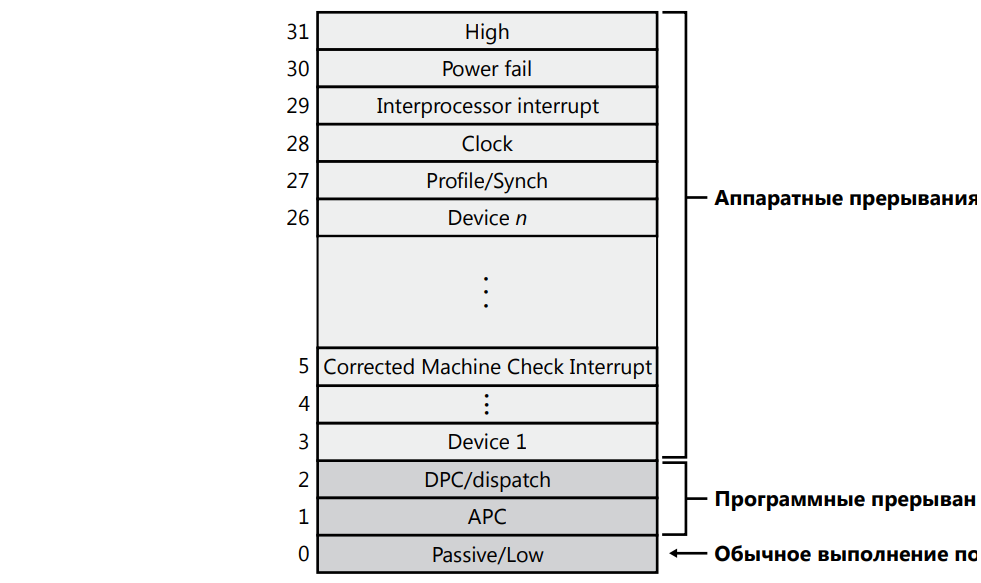
\includegraphics[width=0.85\textwidth]{img/1.png}
	\caption{Уровни запросов прерываний (IRQL) для архитектуры x86}
	\label{fig:x86}
\end{figure} 

\begin{figure}[h]
\centering
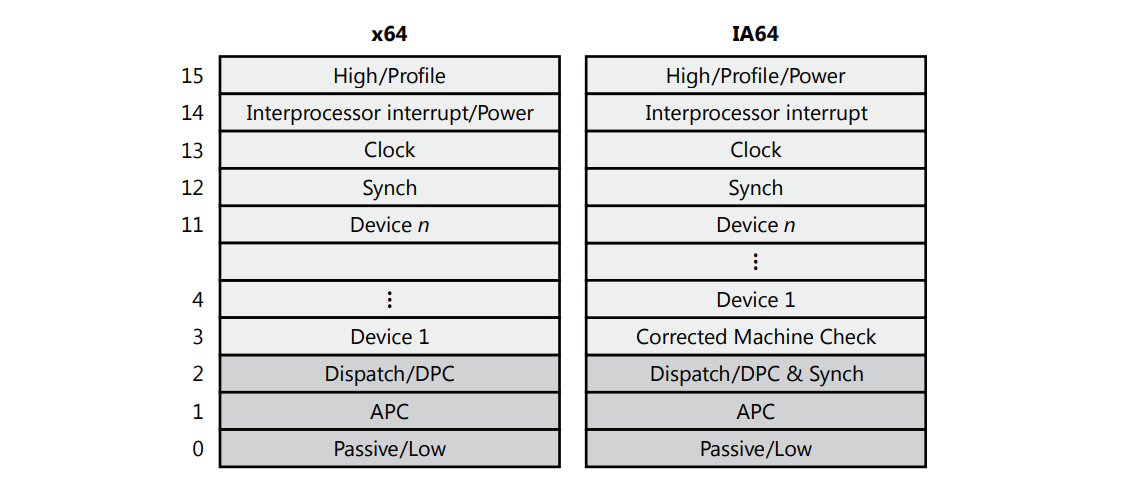
\includegraphics[width=\textwidth]{img/2.png}
\caption{Уровни запросов прерываний (IRQL) для архитектур x64 и IA64}
\label{fig:x64}
\end{figure} 

Прерывания обслуживаются в порядке их приоритета, и прерывания с более высоким уровнем приоритета получают преимущество в обслуживании. При возникновении прерывания с высоким уровнем процессор сохраняет состояние прерванного потока и запускает связанный с прерыванием диспетчер системных прерываний. Тот, в свою очередь, поднимает IRQL и вызывает процедуру обработки прерывания. После выполнения этой процедуры диспетчер прерываний понижает IRQL-уровень процессора до значения, на котором он был до возникновения прерывания, а затем загружает сохраненное состояние машины. Прерванный поток продолжает выполнение с того места, в котором оно было прервано. Когда ядро понижает IRQL, могут реализоваться те прерывания с более низким уровнем приоритета, которые были замаскированы. Если так и происходит, ядро повторяет процесс для обработки новых прерываний.

Уровни приоритетов IRQL имеют совершенно другое значение, чем приоритеты, используемые при планировании потоков. Приоритет планирования является атрибутом потока, а IRQL является атрибутом источника прерывания, такого как клавиатура или мышь. Кроме того, у каждого процессора есть установка IRQL, которая меняется при выполнении кода операционной системы.

Установка IRQL каждого процессора определяет, какие прерывания данный процессор может получать. IRQL-уровни также используются для синхронизации доступа к структуре данных режима ядра. Как только запускается поток режима ядра, он повышает или понижает IRQL процессора либо напрямую, путем вызова функций KeRaiseIrql и KeLowerIrql, либо, что случается чаще, опосредованно, через вызовы функций, которые запрашивают объекты ядра, используемые для синхронизации. Как показано на рисунке \ref{fig:mask}, прерывания, поступающие от источника с IRQL, превышающим текущий уровень, прерывают работу процессора, а прерывания, поступающие от источников с IRQL-уровнями равными или ниже текущего уровня, маскируются до тех пор, пока выполняющийся поток не понизит IRQL.

\clearpage
\begin{figure}[h]
	\centering
	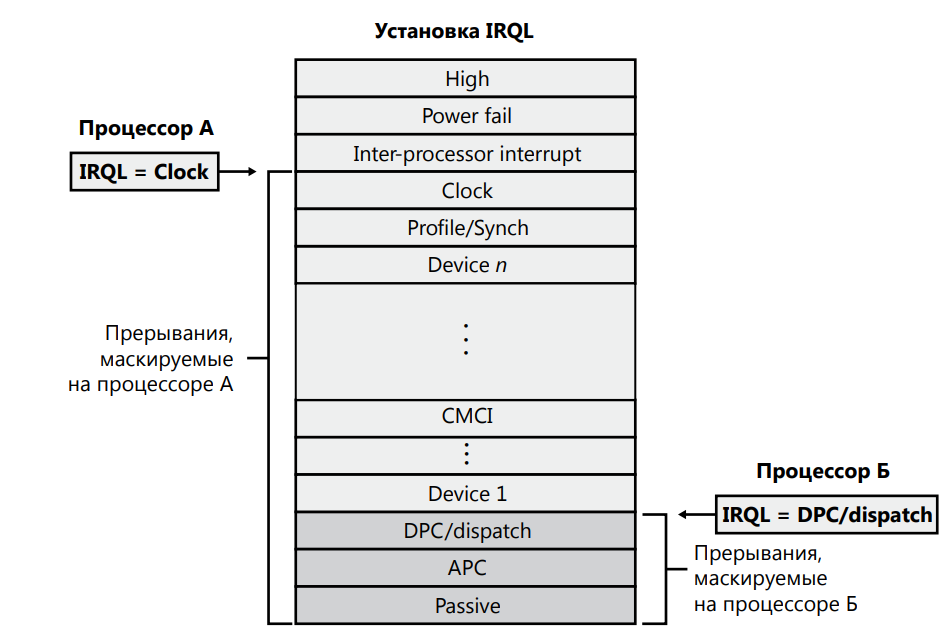
\includegraphics[width=0.83\textwidth]{img/3.png}
	\caption{Маскирование прерываний}
	\label{fig:mask}
\end{figure} 



\subsection{Unix/Linux}

% Unix является изначально многопользовательской и многозадачной системой. В Unix-подобных ОС используется вытесняющая многозадачность. Основным различием между вытесняющим и невытесняющим вариантами многозадачности является степень централизации механизма планирования процессов. В первом случае механизм планирования процессов целиком сосредоточен в операционной системе, а во втором --- распределен между системой и прикладными программами. При невытесняющей многозадачности активный процесс выполняется до тех пор, пока он сам, по собственной инициативе, не отдаст управление операционной системе для того, чтобы та выбрала из очереди другой готовый к выполнению процесс. При вытесняющей многозадачности решение о переключении процессора с одного процесса на другой принимается операционной системой, а не самим активным процессом.

В современном Unix ядро является вытесняющим --- процесс в режиме ядра может быть вытеснен более приоритетным процессом, так же находящимся в режиме ядра. Это было сделано  для того, чтобы система могла обслуживать процессы реального времени, такие как воспроизведение видео или аудио.

Согласно приоритетам процессов и принципу вытесняющего циклического планирования формируется очередь готовых к выполнению потоков. В 
первую очередь выполняются процессы с большим приоритетом. Процессы с одинаковыми приоритетами выполняются в течении кванта времени --- 
циклически, друг за другом. В случае, если поток, имеющий более высокий приоритет поступает в очередь готовых к выполнению процессов, 
планировщик вытесняет текущий процесс и предоставляет ресурс более приоритетному процессу.

Приоритет --- это целое число, находящееся в диапазоне от 0 до 127. Чем меньше значение, тем выше приоритет процесса. Приоритеты ядра 
варьируются от 0 до 49, а приоритеты прикладных задач от 50 до 127. Приоритеты ядра являются статическими величинами, а приоритеты 
прикладных задач могут изменяться во времени в зависимости от двух факторов: фактора <<любезности>> и фактора утилизации.

Фактор <<любезности>> --- это целое число в диапазоне от 0 до 39 (по умолчанию 20). Чем меньше значение фактора <<любезности>> процесса, 
тем выше приоритет процесса. Фактор <<любезности>> процесса может быть изменен с помощью системного вызова \textbf{nice}, но только 
суперпользователем. Фоновым процессам задаются более высокие значения фактора <<любезности>>.

Фактор утилизации определяется последней измеренной величиной использования процессора. Этот фактор позволяет системе динамически изменять приоритет процесса.

Дескриптор процесса \textbf{proc} содержит следующие поля, которые относятся к приоритету процесса:

\begin{itemize}
    \item \textbf{p\_pri} --- текущий приоритет планирования;
    \item \textbf{p\_usrpri} --- приоритет процесса в режиме задачи;
    \item \textbf{p\_cpu} --- результат последнего измерения степени загруженности процессора (процессом);
    \item \textbf{p\_nice} --- фактор любезности, устанавливаемый пользователем.
\end{itemize}

Когда процесс находится в режиме задачи, значения \textbf{p\_pri} и \textbf{p\_usrpri} равны. Значение текущего приоритета \textbf{p\_pri} 
может быть повышено планировщиком для выполнения процесса в режиме ядра, а \textbf{p\_usrpri} будет использоваться для хранения приоритета 
который будет назначение когда процесс вернется в режим задачи.

Ядро системы связывает приоритет сна с событием или ожидаемым ресурсом, из-за которого процесс может блокироваться. В тот момент когда 
процесс просыпается, после того как был блокирован в системном вызове, ядро устанавливается приоритет сна в поле \textbf{p\_pri} --- это 
значение приоритета в диапазоне от 0 до 49, зависящее от события или ресурса по которому произошла блокировка. В таблице \ref{tab:bsd} 
приведены значения приоритетов сна для систем \textbf{4.3BSD}.

\begin{longtable}[Hc]{|p{8.5cm}|p{3.6cm}|p{3.6cm}|}
	\caption{Приоритеты сна в ОС 4.3 BSD\label{tab:bsd}}\\
	\hline
	\textbf{Событие} & \textbf{Приоритет 4.3BSD UNIX} & \textbf{Приоритет SCO UNIX} \\
	\hline
	Ожидание загрузки в память сегмента/страницы & 0 & 95 \\
	\hline
	Ожидание индексного дескриптора & 10 & 88 \\
	\hline
	Ожидание ввода-вывода & 20 & 81 \\
	\hline
	Ожидание буфера & 30 & 80 \\
	\hline
	Ожидание терминального ввода  &  & 75 \\
	\hline
	Ожидание терминального вывода &  & 74 \\
	\hline
	Ожидание завершения выполнения &  & 73 \\
	\hline
	Ожидание события --- низкоприоритетное состояние сна & 40 & 66 \\
	\hline
\end{longtable}

При создании процесса после \textbf{p\_cpu} инициализируется нулём. На каждом тике обработчик таймера увеличивает это поле для текущего 
процесса на единицу, до максимального значения, которое равно 127. Каждую секунду обработчик прерывания инициализирует отложенный вызов 
процедуры \textbf{schedcpy()}, которая уменьшает значение \textbf{p\_cpu} каждого процесса исходя из фактора <<полураспада>>. В системе 
\textbf{4.3BSD} фактор полураспада рассчитывается по формуле \eqref{for:bsd}: 

\begin{equation}
    \label{for:bsd}
    decay = \frac{2 \cdot load\_average}{2 \cdot load\_average + 1}
\end{equation}
где \textbf{load\_average} --- среднее количество процессов, находящихся в состоянии готовности к выполнению (за последнюю секунду).

Приоритеты для режима задачи всех процессов в процедуре \textbf{schedcpy()} пересчитываются по формуле \eqref{for:sched}:

\begin{equation}
    \label{for:sched}
    p\_usrpri = PUSER + \frac{p\_cpu}{4} + 2 \cdot p\_nice
\end{equation}
где \textbf{PUSER} --- базовый приоритет в режиме задачи, равный 50.

Если процесс в последний раз использовал большое количество процессорного времени, его \textbf{p\_cpu} будет увеличен. Это приведёт к 
росту значения \textbf{p\_usrpri} и понижению приоритета. Чем дольше процесс находится в очереди на исполнение, тем больше 
фактор полураспада уменьшает его \textbf{p\_cpu}, что приводит к повышению его приоритета. Данная схема предотвращает бесконечное откладывание 
низкоприоритетных процессов. Применение такой схемы более предпочтительно для процессов, которые осуществляют много 
операций ввода-вывода, и менее предпочтительно для процессов, производящих много вычислений.

\section*{Заключение}
Обработчики прерывания от системного таймера в защищенном режиме в системах Unix и Windows выполняют одинаковые действия:

\begin{itemize} 
	\item выполняют декремент счетчиков времени: таймеров, счетчиков времени отложенных действий, будильников реального времени;
	\item выполняют декремент кванта текущего процесса в Linux и декремент текущего потока в Windows;
	\item инициализируют отложенные действия, относящиеся к работе планировщика, такие как пересчёт приоритетов.
\end{itemize} 

Обе системы являются системами разделения времени с динамическими приоритетами и вытеснением процессов. Такой подход позволяет 
поддерживать процессы реального времени, такие как воспроизведение аудио и видео. Пересчёт динамических приоритетов пользовательских 
процессов выполняется для того, чтобы не допустить их бесконечного откладывания.



\end{document}
